%!TEX root = main.tex

\section{Convexity}
\sectionlabel{convexity}

This lecture provides the most important facts about convex sets and convex
functions that we'll heavily make use of. When $f$ is sufficiently smooth, these are often simple consequences of
Taylor's theorem. 

\subsection{Convex sets}

\begin{definition}[Convex set]
A set $K\subseteq\R^n$ is \emph{convex} if it the line segment between any two points in~$K$ is also contained in~$K.$ Formally, for all $x,y\in K$ and all scalars $\gamma\in[0,1]$ we have $\gamma x+(1-\gamma)y\in K.$
\end{definition}

\begin{theorem}[Separation Theorem]
\theoremlabel{separation}
Let $C, K\subseteq\R^n$ be convex sets with empty intersection $C\cap K=\emptyset.$ Then there exists a point $a\in\R^n$ and a number $b\in\R$ such that
\begin{enumerate}
\item for all $x\in C,$ we have $\langle a, x\rangle \ge b.$
\item for all $x\in K,$ we have $\langle a, x\rangle \le b.$
\end{enumerate}
If $C$ and $K$ are closed and at least one of them is bounded, then we can replace the inequalities by strict inequalities.
\end{theorem}
The case we're most concerned with is when both sets are compact (i.e., closed and bounded). We highlight its proof here.
\begin{proof}[Proof of \theoremref{separation} for compact sets.]
In this case, the Cartesian product $C\times K$ is also compact. Therefore, the
distance function $\|x-y\|$ attains its minimum over $C\times K.$ Taking $p, q$
to be two points that achieve the minimum. A separating hyperplane is given by
the hyperplane perpendicular to $q-p$ that passes through the midpoint between
$p$ and $q.$ That is, $a=q-p$ and $b=(\langle a, q\rangle - \langle a,
p\rangle)/2.$ For the sake of contradiction, suppose there is a point~$r$ on
this hyperplane contained in one of the two sets, say,~$C.$ Then the line
segment from $p$ to $r$ is also contained in~$C$ by convexity. We can then find
a point along the line segment that is close to $q$ than $p$ is, thus
contradicting our assumption.
\end{proof}

\subsubsection{Notable convex sets}
\begin{itemize}
\item Linear spaces $\{x\in\R^n\mid Ax=0\}$ and halfspaces $\{x\in\R^n \mid \langle a, x\rangle \ge 0 \}$
\item Affine transformations of convex sets. If $K\subseteq\R^n$ is convex, so is $\{Ax+b\mid x\in K\}$ for any $A\in\R^{m\times n}$ and $b\in\R^m.$
In particular, affine subspaces and affine halfspaces are convex.
\item Intersections of convex sets. In fact, every convex set is equivalent to the intersection of all affine halfspaces that contain it (a consequence of the separating hyperplane theorem).
\item The cone of positive semidefinite matrices, denotes, $S^n_+ = \{ A\in\R^{n\times n}\mid A\succeq 0\}.$ Here we write $A\succeq 0$ to indicate that $x^\trans A x\ge 0$ for all $x\in\R^n.$ The fact that $S^n_+$ is convex can be verified directly from the definition, but it also follows from what we already knew. 
Indeed, denoting by $S_n=\{A\in\R^{n\times n}\mid A^\trans = A\}$ the set of all $n\times n$ symmetric matrices, we can write $S^n_+$ as an (infinite) intersection of halfspaces $S^n_+=\bigcap_{x\in\R^n\backslash\{0\}} \{ A\in S_n\mid x^\trans A x\ge 0\}.$
\item See Boyd-Vandenberghe for lots of other examples.
\end{itemize}

\subsection{Convex functions}

\begin{definition}[Convex function]
A function $f\colon\domain\to\R$ is \emph{convex} if for all $x,y\in\domain$ and all scalars $\gamma\in[0,1]$ we have $f(\gamma x+(1-\gamma)y)\le \gamma f(x)+(1-\gamma)f(y).$
\end{definition}

Jensen (1905) showed that for continuous functions, convexity follows from the ``midpoint'' condition that for all $x,y\in\domain,$
\[
f\left(\frac{x+y}2\right)\le \frac{f(x)+f(y)}2\,.
\]
This result sometimes simplifies the proof that a function is convex in cases where we already know that it's continuous.

\begin{figure}
\begin{center}
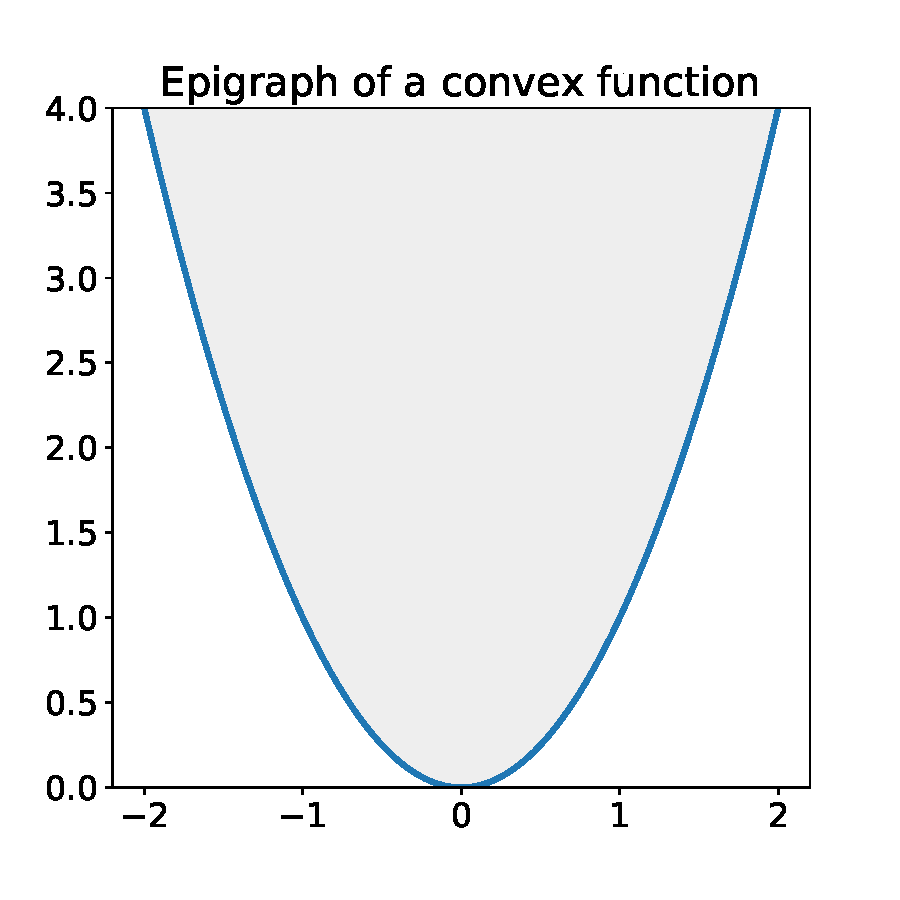
\includegraphics[width=3in]{figures/lecture1-epigraph}
\end{center}
\end{figure}
\begin{definition}

The \emph{epigraph} of a function~$f\colon \domain\to\R$ is defined as 
\[
\epi(f) = \{(x, t)\mid f(x)\le t\}\,.
\]
\end{definition}

\begin{fact}
A function is convex if and only if its epigraph is convex.
\end{fact}

Convex functions enjoy the property that local minima are also global minima. Indeed, suppose that $x\in\domain$ is a local minimum of~$f\colon\domain\to\R$ meaning that any point in a neighborhood around $x$ has larger function value. Now, for every $y\in\domain,$ we can find a small enough $\gamma$ such that
\[
f(x) \le f((1-\gamma)x+\gamma y) \le (1-\gamma)f(x)+\gamma f(y)\,.
\]
Therefore, $f(x)\le f(y)$ and so $x$ must be a global minimum.

\subsubsection{First-order characterization}

It is helpful to relate convexity to Taylor's theorem, which we recall now. We define the \emph{gradient} of a differentiable function~$f\colon\domain\to\R$ at $x\in\domain$ as the vector of partial derivatives
\[
\nabla f(x) = \left( \frac{\partial f}{\partial x_i} \right)_{i=1}^n\,.
\]
We note the following simple fact that relates linear forms of the gradient to a
one-dimensional derivative evaluated at~$0.$ It's a consequence of the multivariate chain rule.
\begin{fact}
\factlabel{1d-nd-gradient}
Assume $f\colon\domain\to\R$ is differentiable and let $x,y\in\domain.$ Then,
\[
\nabla f(x)^\trans y
= \left.\frac{\partial f(x+\gamma y)}{\partial \gamma}\right|_{\gamma=0}\,.
\]
\end{fact}
Taylor's theorem implies the following statement.
\begin{proposition}
\propositionlabel{first-order-taylor}
Assume $f\colon\domain\to\R$ is continuously differentiable along the line segment between two points $x$ and $y.$ Then,
\[
f(y) = f(x) 
+ \nabla f(x)^\trans (y-x)
+ \int_0^1 (1-\gamma)\frac{\partial^2 f(x+\gamma(y-x))}{\partial\gamma^2}\rd\gamma
\]
\end{proposition}
\begin{proof}
Apply a second order Taylor's expansion to $g(\gamma)=f(x+\gamma(y-x))$ and apply \factref{1d-nd-gradient} to the first-order term. 
\end{proof}

Among differentiable functions, convexity is equivalent to the property that the first-order Taylor approximation provides a global lower bound on the function.

\begin{figure}
\begin{center}
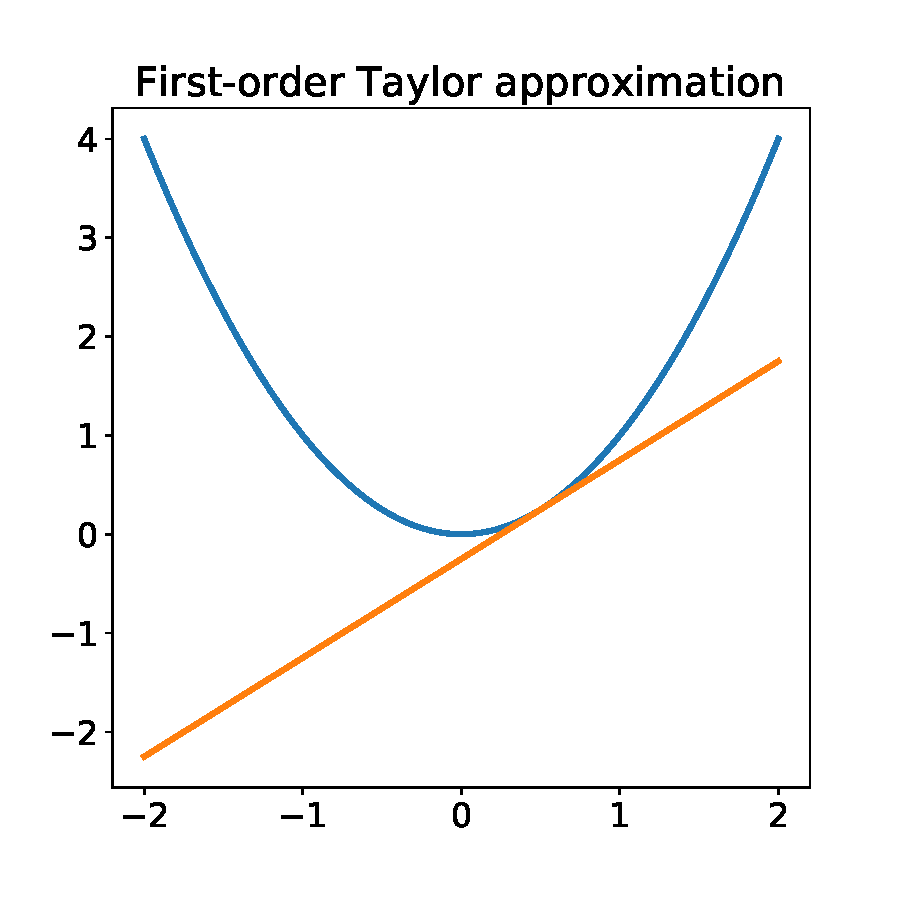
\includegraphics[width=3in]{figures/lecture1-taylor}
\end{center}
\caption{Taylor approximation of $f(x)=x^2$ at $0.5.$}
\end{figure}

\begin{proposition}
\propositionlabel{first-order-lower-bound}
Assume $f\colon\domain\to\R$ is differentiable. Then, $f$ is convex if and only if for all $x,y\in\domain$ we have
\begin{equation}\equationlabel{first-order-lower-bound}
f(y) \ge f(x) + \nabla f(x)^\trans (y-x)\,.
\end{equation}
\end{proposition}
\begin{proof}
First, suppose $f$ is convex, then by definition
\begin{align*}
f(y) &\ge \frac{f((1-\gamma)x+\gamma y)-(1-\gamma)f(x)}{\gamma}\\
&\ge f(x) +\frac{f(x+\gamma(y-x))-f(x)}\gamma\\
&\rightarrow f(x) +\nabla f(x)^\trans (y-x) \quad\text{as $\gamma\to 0$} \tag{by \factref{1d-nd-gradient}.}
\end{align*}
On the other hand, fix two points $x, y\in\domain$ and $\gamma\in[0,1]$. Putting $z=\gamma x + (1-\gamma)y$ we get from applying \equationref{first-order-lower-bound} twice,
\[
f(x) \ge f(z) + \nabla f(z)^\trans (x-z)
\quad\text{and}\quad
f(y) \ge f(z) + \nabla f(z)^\trans (y-z)
\]
Adding these inequalities scaled by $\gamma$ and $(1-\gamma)$, respectively, we get $\gamma f(x)+(1-\gamma)f(y)\ge f(z),$ which establishes convexity.
\end{proof}

A direct consequence of \propositionref{first-order-lower-bound} is that
if $\nabla f(x)=0$ vanishes at a point~$x,$ then $x$ must be a global minimizer
of~$f.$

\begin{remark}[Subgradients]
Of course, not all convex functions are differentiable. The absolute
value~$f(x)=|x|,$ for example, is convex but not differentiable at $0.$
Nonetheless, for every $x,$ we can find a vector $g$ such that
\[
f(y) \ge f(x) + g^\trans (y-x)\,.
\]
Such a vector is called a \emph{subgradient} of $f$ at $x.$ The existence of
subgradients is often sufficient for optimization.
\end{remark}

\subsubsection{Second-order characterization}

We define the \emph{Hessian} matrix of $f\colon\domain\to\R$ at a point $x\in\domain$ as the matrix of second order partial derivatives:
\[
\nabla^2 f(x) = \left( \frac{\partial^2 f}{\partial x_i\partial x_j} \right)_{i,j\in[n]}\,.
\]
Schwarz's theorem implies that the Hessian at a point $x$ is symmetric provided
that $f$ has continuous second partial derivatives in an open set around~$x.$

In analogy with \factref{1d-nd-gradient}, we can relate quadratic forms in the
Hessian matrix to one-dimensional derivatives using the chain rule.
\begin{fact}
\factlabel{1d-nd-hessian}
Assume that $f\colon\domain\to\R$ is twice differentiable along the line segment from $x$ to $y.$ Then,
\[
y^\trans \nabla^2f(x+\gamma y)y 
= \frac{\partial^2f(x+\gamma y)}{\partial\gamma^2}\,.
\]
\end{fact}

\begin{proposition}
If $f$ is twice continuously differentiable on its domain~$\domain$, then $f$ is convex if and only if $\nabla^2 f(x)\succeq 0$ for all $x\in\domain.$ 
\end{proposition}
\begin{proof}
Suppose $f$ is convex and our goal is to show that the Hessian is positive semidefinite. 
Let $y=x + \alpha u$ for some arbitrary vector~$u$ and scalar $\alpha.$
\propositionref{first-order-lower-bound} shows
\[
f(y) - f(x) -\nabla f(x)^\trans (y-x) \ge 0
\]
Hence, by \propositionref{first-order-taylor},
\begin{align*}
0&\le  \int_0^1 (1-\gamma)\frac{\partial^2 f(x+\gamma(y-x))}{\partial\gamma^2}\rd\gamma\\
&=  (1-\gamma)\frac{\partial^2 f(x+\gamma(y-x))}{\partial\gamma^2}
\quad\text{for some $\gamma\in(0,1)$} \tag{by the mean value theorem}\\
&= (1-\gamma)(y-x)^\trans \nabla^2 f(x+\gamma (y-x))(y-x) 
\tag{by \factref{1d-nd-hessian}}\,.
\end{align*}
Plugging in our choice of~$y,$ this shows $0\le u^\trans \nabla^2
f(x+\alpha\gamma u)u.$ Letting $\alpha$ tend to zero establishes that $\nabla^2
f(x)\succeq 0.$ (Note that $\gamma$ generally depends on $\alpha$ but is always
bounded by~$1.$)

Now, suppose the Hessian is positive semidefinite everywhere in $\domain$ and
our goal is to show that  the function~$f$ is convex.  Using the same derivation
as above, we can see that the second-order error term in Taylor's theorem must
be non-negative. Hence, the first-order approximation is
a global lower bound and so the function~$f$ is convex by
\propositionref{first-order-lower-bound}.
\end{proof}

\subsection{Convex optimization}
Much of this course will be about different ways of minimizing a convex function~$f\colon\domain\to\R$ over a convex domain~$\domain:$ 
\[
\min_{x\in\domain}\quad f(x)
\]
Convex optimization is not necessarily easy! 
For starters, convex sets do not necessarily enjoy compact descriptions. When solving computational problems involving convex sets, we need to worry about how to represent the convex set we're dealing with. Rather than asking for an explicit description of the set, we can instead require a computational abstraction that highlights essential operations that we can carry out. The Separation Theorem motivates an important computational abstraction called \emph{separation oracle}.

\begin{definition}
A \emph{separation oracle} for a convex set~$K$ is a device, which given any
point $x\not\in K$ returns a hyperplane separating $x$ from $K.$
\end{definition}

Another computational abstraction is a \emph{first-order oracle} that given a
point $x\in\domain$ returns the gradient $\nabla f(x).$ Similarly, a
\emph{second-order oracle} returns $\nabla^2 f(x).$ A function value oracle or
\emph{zeroth-order oracle} only returns $f(x).$ First-order methods are
algorithms that make do with a first-order oracle.  Analogously, we can define
zeroth-order method, and second-order method.

\subsubsection{What is efficient?}
Classical complexity theory typically quantifies the resource consumption
(primarily running time or memory) of an algorithm in terms of the bit
complexity of the input. We say things like ``we can multiply two $n$-bit
numbers in time $O(n^2)$ using long multiplication method.''

This computational approach can be cumbersome in convex optimization and most
textbooks shy away from it. Instead, it's customary in optimization to quantify
the cost of the algorithm in terms of more abstract resources, like, how often
it accesses one of the oracles we mentioned. Counting oracle can give us a rough
sense of how well we expect a method to work.

The definition of ``efficient'' is not completely cut and dry in optimization.
Typically, our goal is to show that an algorithm finds a solution~$x$ with 
\[
f(x) \le \min_{x\in\domain}f(x) + \epsilon
\]
for some additive error $\epsilon>0.$ 
The
cost of the algorithm will depend on the target error.  Highly practical
algorithms often have a polynomial dependence on $\epsilon,$ such as
$O(1/\epsilon)$ or even $O(1/\epsilon^2).$ Other algorithms achieve
$O(\log(1/\epsilon))$ steps in theory, but are prohibitive in their actual
computational cost. Technically, if we think of the parameter~$\epsilon$ as
being part of the input, it takes only $O(\log(1/\epsilon))$ bits to describe
the error parameter. Therefore, an algorithm that depends more than
logarithmically on $1/\epsilon$ may not be polynomial time algorithm in its
input size.

In this course, we will make an attempt to highlight both the theoretical performance and practical appeal of an algorithm. Moreover, we will discuss other performance criteria such as robustness to noise. How well an algorithm performs is rarely decided by a single criterion, and usually depends on the application at hand.
